\section*{Question 5:}
Exercise 7.2: 

Can you think of another measure of similarity that could be used in the vector space model? Compare your measure with the cosine correlation using some example documents and queries with made-up weights. Browse the IR literature on the Web and see whether your measure has been studied (start with van Rijsbergen’s book).

\subsection*{Answer:}

In order for the similarity measure to give correct results when used in the vector space model, it must be based on the angle between the vectors. Any measure that is based on the Euclidean distance will give wrong results unless vectors, query \& documents' vectors, are reduced to the unit vectors, which is what cosine similarity does.

\textbf{Example:}

We have a query q = ``Do jealous people gossip?''. Let's assume that the two terms ``do'' and ``people'' are stop words. The two terms that affect the results are ``jealous'' and ``gossip''.

We also have three documents to examine, $d_1$, $d_2$, and $d_3$.

$d_1$: A document that is mostly about gossip, but has a little about jealousy.

$d_2$: A document about both gossip and jealousy. It has a little more about jealousy than it does about gossip. It is the most relevant document out of all three documents.

$d_3$: A document that is mostly about jealousy, but has a little about gossip.

Euclidean distance similarity will cause $d_1$ and $d_3$ to be ranked higher than $d_2$ with respect to the query q because the distance between q and $d_2$ is larger than the distance between q and $d_1$ as well as the distance between q and $d_3$. The result is clear in Figure 7 and Figure 8.

\begin{figure}[h]
\caption{Euclidean Distance Similarity Between Vectors}
\centering
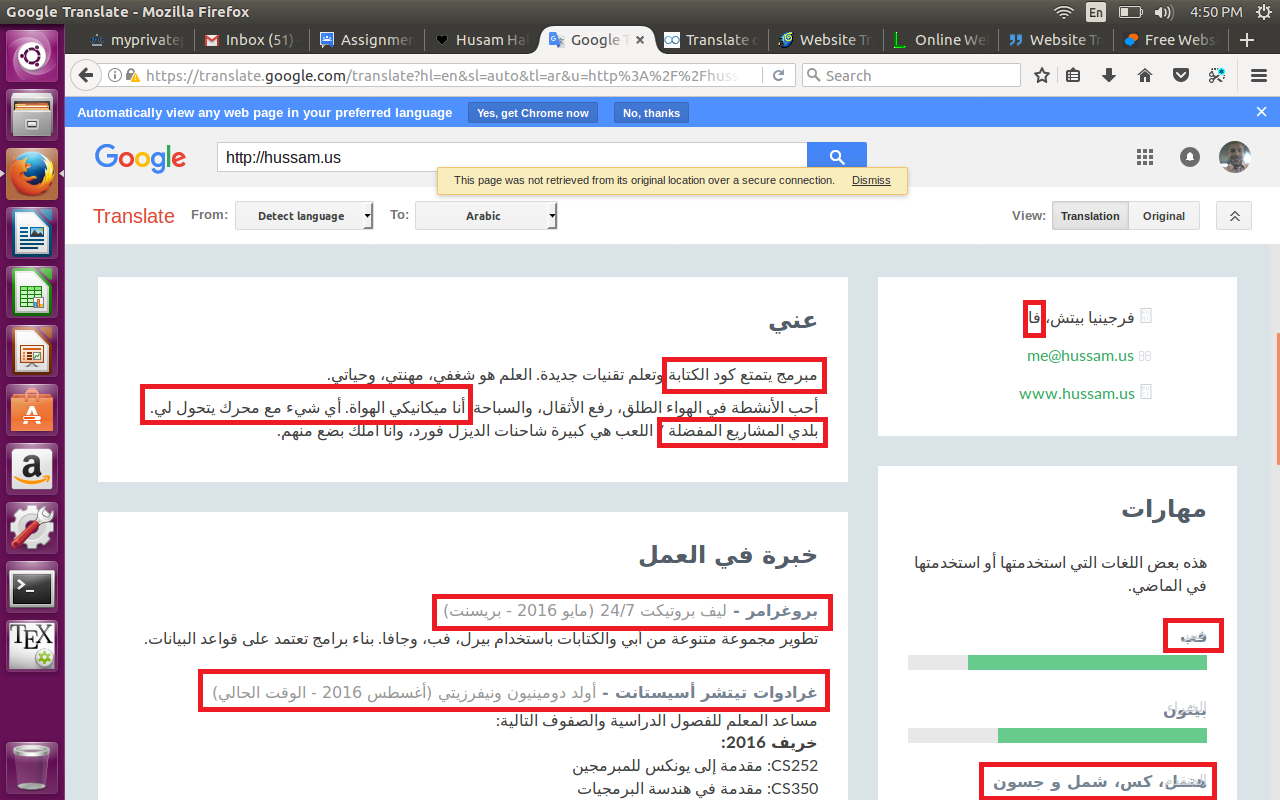
\includegraphics[scale=0.7]{Q5/1.png}
\end{figure}


\begin{figure}[h]
\caption{Euclidean Distance Similarity Between Vectors}
\centering
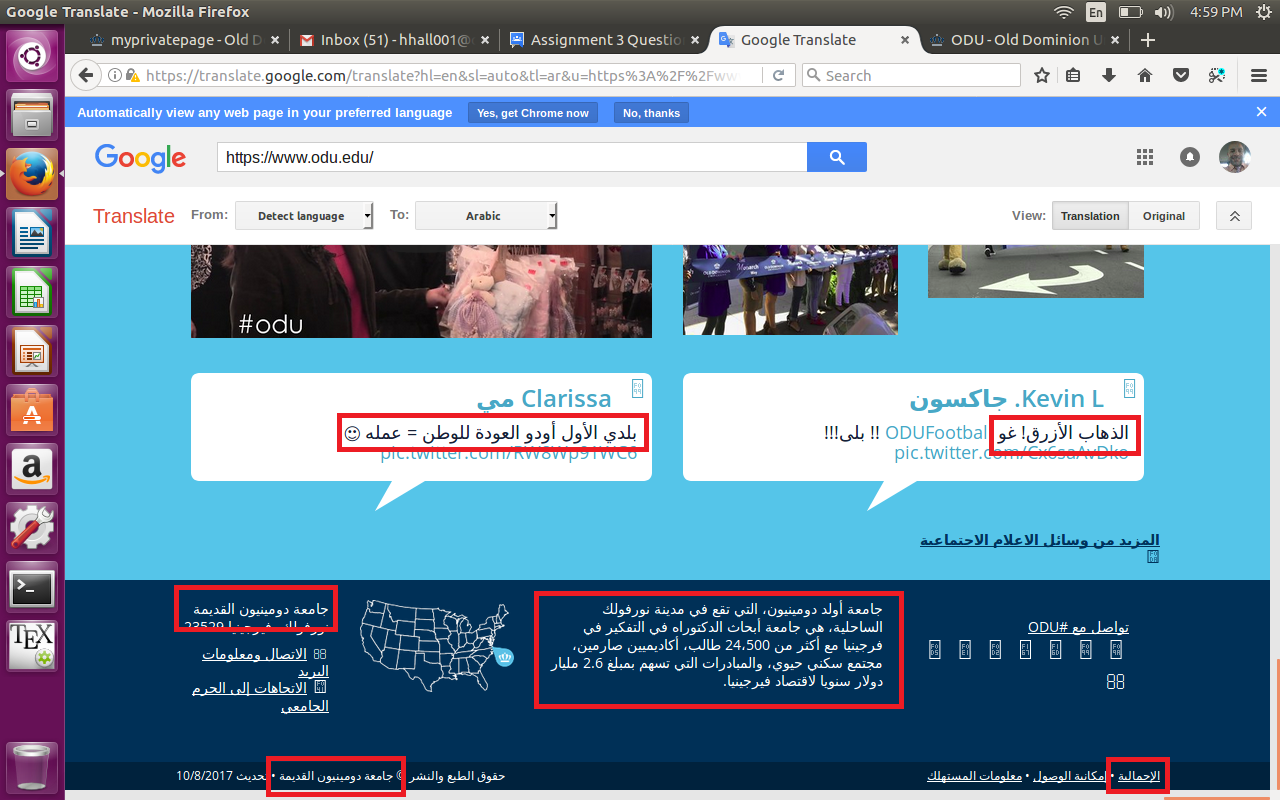
\includegraphics[scale=0.6]{Q5/2.png}
\end{figure}


The only case where Euclidean distance can be used as a similarity measure is when all vectors are reduced to the unit vector. This reduction can be performed by dividing each component in the vector by the vector's magnitude. The result is clear in Figure 9.

\begin{figure}[h]
\caption{Euclidean Distance Similarity Between Unit Vectors}
\centering
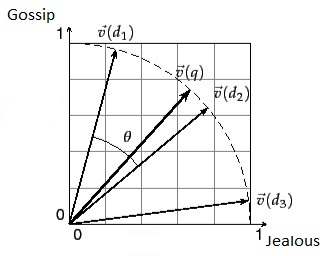
\includegraphics[scale=0.8]{Q5/4.jpg}
\end{figure}


\begin{figure}[h]
\caption{Cosine Similarity Between Vectors}
\centering
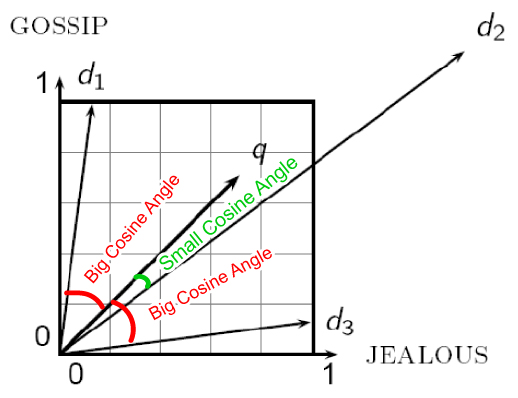
\includegraphics[scale=0.6]{Q5/3.jpg}
\end{figure}



The cotangent of the angle between vectors could be used as a measure of similarity in the vector space model. Cotangent $\theta$ is the reciprocal of tangent $\theta$. The graph of the function $y = cot(x)$ is shown in Figure 11.

\begin{figure}[h]
\caption{The graph of the function $y = cot(x)$}
\centering
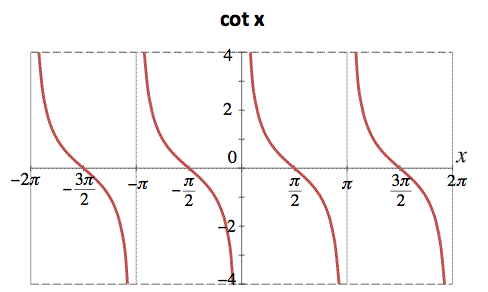
\includegraphics[scale=1.1]{Q5/graph_cot_pi.png}
\end{figure}


The period of the function cotangent that should be used lies in the interval $\theta = [0,\pi]$

From the graph, three statements can be made:

1. If the angle between the vectors is zero, the value of the cotangent is $\infty$.

2. If the angle between the vectors is $\frac{\pi}{2}$, the value of the cotangent is zero.

3. If the angle between the vectors is $\pi$, the value of the cotangent is $-\infty$.

This similarity measure agrees with the cosine similarity measure, but it is very steep since its value spans the interval $(-\infty,+\infty)$.

The log function can be wrapped around the cotangent function to reduce its aggression. 

$ similarity = \log_{10} (\cot(\theta))$

The base of the log is not important. Base 10 is not empirically determined. The base is there for completeness.

\textbf{Example with made-up weights:}

Let $q(8,9)$, $d_1(0,9)$, $d_2(25,25)$, and $d_1(9,0)$:

$$cos(q,d_1) = \frac{81}{108.374351209} = 0.747409319$$
$$\theta(q,d_1) = 41.63353931$$

$$cos(q,d_2) = \frac{425}{425.734659152} = 0.998274373$$
$$\theta(q,d_2) = 3.36646083$$

$$cos(q,d_3) = \frac{72}{108.374351209} = 0.664363839$$
$$\theta(q,d_3) = 48.36646065$$

$$log_{10}(cot(q,d_1)) = log_{10}(1.125) = 0.051152522$$

$$log_{10}(cot(q,d_2)) = log_{10}(17) = 1.230448921$$

$$log_{10}(cot(q,d_3)) = log_{10}(0.8889) = -0.051147094$$

\begin{longtable}{ |p{3cm}|p{3cm}|p{3cm}|p{3cm}| } 
\caption{Logarithmic Cotangent and Cosine Similarity Measures}\\    %%%%<===
\hline
Measure & $d_1$ & $d_2$ & $d_3$ \\
 \hline 
 Cosine & 0.747409319 & 0.998274373 & 0.664363839 \\
 \hline
  $log(cot)$ & 0.051152522 & 1.230448921 & -0.051147094 \\
 \hline
\end{longtable}

From the results, we can see that my measure agrees with the cosine correlation measure. The only noticeable difference is that the logarithmic cotangent correlation measure produced a negative value for the similarity between q and $d_3$. This negative result makes sense to a certain extent because $d_3$ is the document that is least related to q according to the results from the cosine similarity measure. My measure ranked the documents by their relevance to the query q as: $d_2, d_1, d_3$. The cosine correlation measure produced the same ranking.



 
